\documentclass{article}
\usepackage[utf8]{inputenc}

\usepackage{tikz}
\usetikzlibrary{shapes}
\begin{document}
\begin{center}
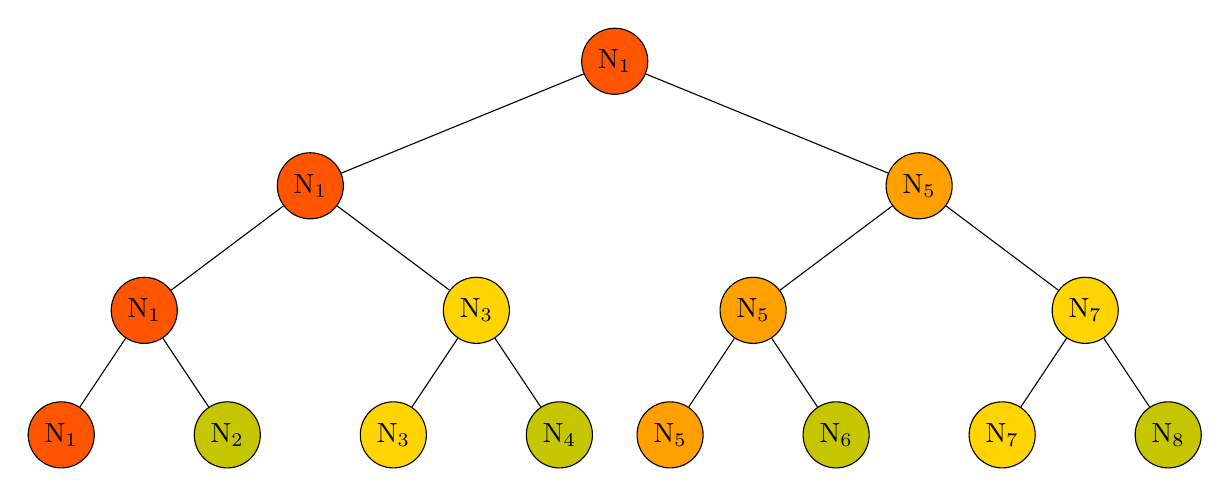
\begin{tikzpicture}[
  level distance=45 pt,
  inner/.style={fill={rgb:red,1;green,0;yellow,5},circle,draw}, % nodes are circles
  middle/.style={fill={rgb:red,3;green,0;yellow,5},circle,draw},
  outer/.style={fill={rgb:red,10;green,0;yellow,5},circle,draw},
  ouyer/.style={fill={rgb:red,2;green,2;yellow,5},circle,draw},
  level 1/.style={sibling distance=220 pt},
  level 2/.style={sibling distance=120 pt},
  level 3/.style={sibling distance=60 pt}
]
 
  \node [outer]{$\mathrm{N}_1$}
    child {node [outer]{$\mathrm{N}_1$}
      child {node [outer]{$\mathrm{N}_1$}
        child {node[outer]{$\mathrm{N}_1$}}
        child {node[ouyer]{$\mathrm{N}_2$}}
      }
      child {node[inner]{$\mathrm{N}_3$}
        child {node[inner]{$\mathrm{N}_3$}}
        child {node[ouyer]{$\mathrm{N}_4$}}
      }
     }
    child {node [middle]{$\mathrm{N}_5$}
      child {node [middle]{$\mathrm{N}_5$}
        child {node[middle]{$\mathrm{N}_5$}}
        child {node[ouyer]{$\mathrm{N}_6$}}
      }
      child {node[inner]{$\mathrm{N}_7$}
        child {node[inner]{$\mathrm{N}_7$}}
        child {node[ouyer]{$\mathrm{N}_8$}}
      }
    };
    
\end{tikzpicture}\end{center}

\end{document}
